\section{Basis Word Encoding Strategy}\label{sec:basis_words}

The encoding of the basis set for representation of the sentence states requires several key steps:
\begin{itemize}
    \item Tokenise corpus, and tag with appropriate meaning-space type using the `NLTK' Python library.
    \item Separate tokens into noun and verb datasets.
    \item Define basis tokens in each set as $n$-most frequent tokens.
    \item Map basis token to binary strings, using a given encoding scheme.
    \item Project composite words (i.e. non-basis words) onto basis word set for encoding meanings.
\end{itemize}

To ensure the mapping of the basis words to encoding pattern is reflective of the underlying distributional distances between words in the corpus, it is necessary to choose an encoding scheme such that the inter-token relationships are preserved. For this, we choose a simplified encoding scheme where the Hamming distance between each bit-string is equal to the distance between the bit-strings in the data set. This can easily be created by left-shifting $1$'s into the register until full, then outwards. For 2 and 4-qubit registers respectively, this would equate to the patterns
\begin{align*}
    p_2 &\in \{00,\, 01,\, 11,\, 10\}, \\
    p_4 &\in \{0000,\, 0001,\, 0011,\, 0111,\, 1111,\, 1110,\, 1100,\, 1000 \},
\end{align*}
of which $p_n$ can be extrapolated to from the above model.

Given these encoding patterns, we can show the Hamming distances between each pattern and others in the set have a well-defined position-to-distance relationship. The example given by Fig.~\ref{fig:2q_example_encoding} is the method applied to the previous example of ``John rests inside, and Mary walks outside'' from D2.1. We can similarly extend this method to larger datasets, though the ordering problem requires a more automated approach.

\begin{figure}[htbp]
     \centering
     \begin{subfigure}[b]{0.45\textwidth}
         \centering
         \includegraphics[width=\textwidth]{Images/2qubitreg_graph_bitstrings.pdf}
         \caption{}
         \label{fig:2qreg_basis}
     \end{subfigure}
     \hspace{1ex}
     \unskip\ \vrule
     \hspace{1ex}
     \begin{subfigure}[b]{0.45\textwidth}
         \centering
         \includegraphics[width=\textwidth]{Images/2qubitreg_graph_maryjohn.pdf}
         \caption{}
         \label{fig:2qreg_basis}
     \end{subfigure}
        \caption{(a) The simplified encoding scheme defined as a graph, with edges representing the Hamming distances between each respective bit-string. (b) The simplified encoding scheme defined as a graph for the example given in D2.1, where the bit-strings are now associated with a given basis token. The respective similarity between the words in this example is reflected in the given distances. }
        \label{fig:2q_example_encoding}
\end{figure}

\begin{figure}[htbp]
    \centering
    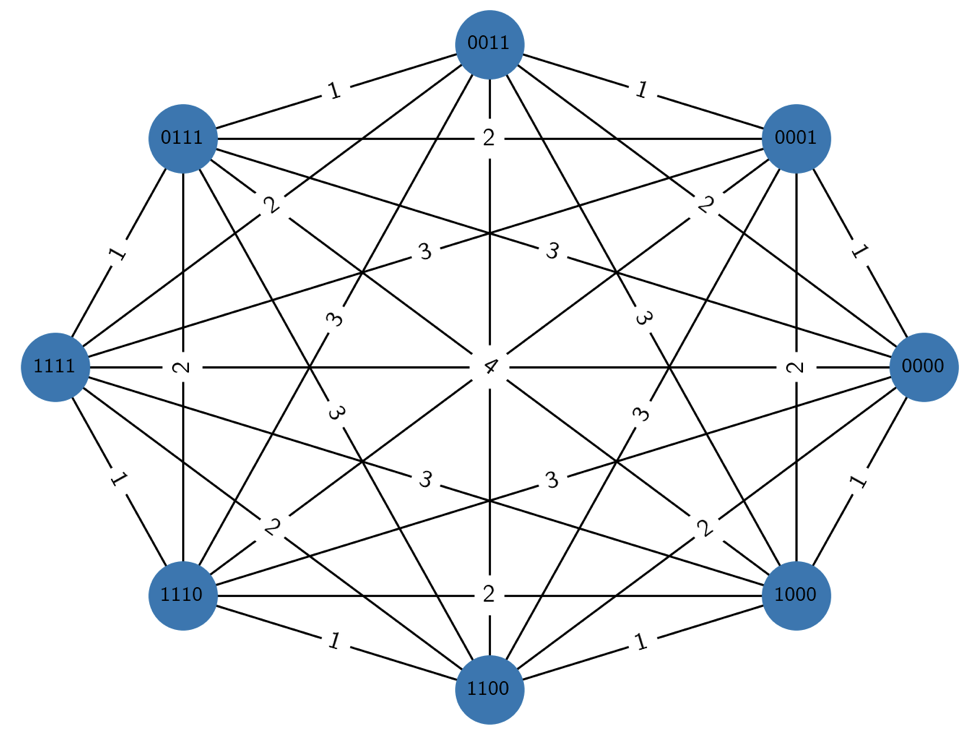
\includegraphics[width=0.6\textwidth]{Images/4qubitreg_graph_bitstrings.png}
    \caption{The graph of the given encoding scheme where the outer ordering of the bit-strings follow the Hamming distance.}
    \label{fig:4q_example_encoding}
\end{figure}

For the 4-qubit encoding scheme, we obtain a fully connected graph as defined by Fig.~\ref{fig:4q_example_encoding}, where again the respective positions of the bit-strings reflect the Hamming distance between them. To effectively map a computationally determined basis to these bit-strings, we use the following procedure:

\begin{itemize}
    \item Given the chosen basis tokens, and their positions in the text, create a graph where each basis token is a single node.
    \item Calculate the distances between all token positions given a pairing of each token with the others ($n*(n-1)/2$ pairings).
    \item For simplicity, choose the minimum distances between each of the pairings, and create edges with this as the given weight. [Note: alternative methods can also be used: mean, median, etc]
    \item With the given fully-connected graph, find a Hamiltonian cycle, and use the returned ordering to map the tokens onto the bit-strings.
\end{itemize}

For any given Hamiltonian cycle, the relationships between each of the tokens will be preserved, and can effectively be mapped onto the bit-string encodings. It can be noted that alternative encoding schemes, and distance orderings could potentially be investigated, but will remain beyond the scope of this current project. Using the above scheme and method, we have determined a given ordering for an 8-basis bit-string set from Lewis Carroll's ``Alice in Wonderland'' as:
\begin{equation}
\begin{array}{cccccc}
\textrm{Alice} & \rightarrow & \vert 0000\rangle, & \textrm{Hatter} & \rightarrow &\vert 0001\rangle, \\
\textrm{King} & \rightarrow & \vert 0011 \rangle, & \textrm{Queen} & \rightarrow &\vert 0111\rangle, \\
\textrm{time} & \rightarrow & \vert 1111 \rangle, &\textrm{Mock} & \rightarrow &\vert 1110\rangle, \\
\textrm{Turtle} & \rightarrow & \vert 1100\rangle, &\textrm{Gryphon} & \rightarrow &\vert 1000\rangle.
\end{array}
\label{eq:aiw_order}
\end{equation}
 with the resulting graph order mapped onto the Fig.~\ref{fig:4q_example_encoding} structure shown by Fig.~\ref{fig:4q_aiw}.

\begin{figure}[htbp]
    \centering
    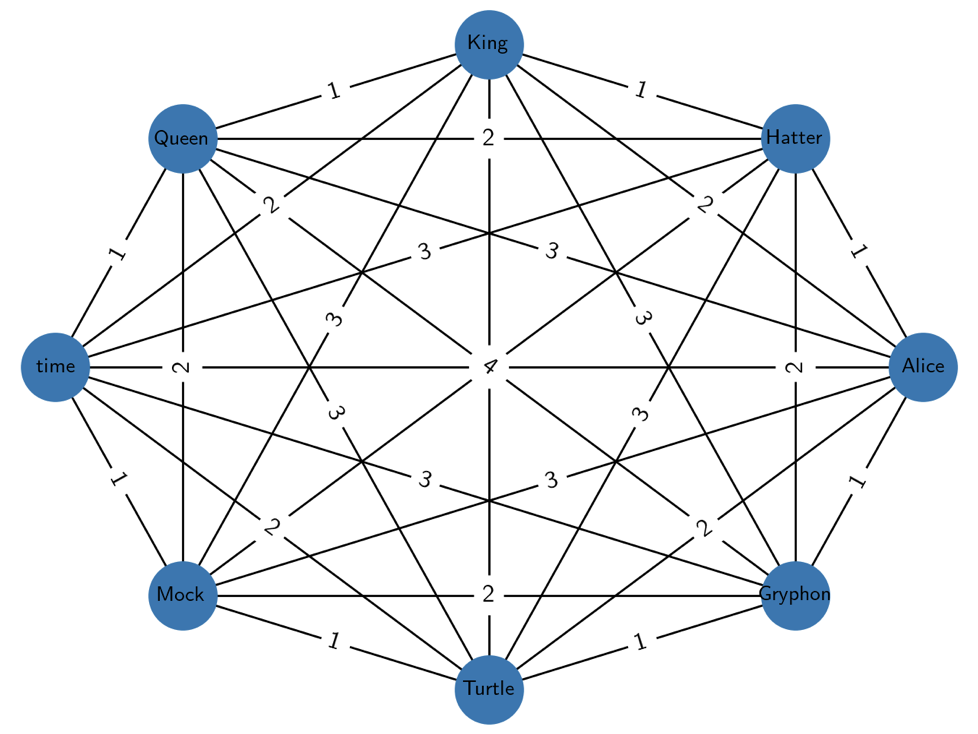
\includegraphics[width=0.6\textwidth]{Images/4qubitreg_graph_aiw.png}
    \caption{Relative ordering of an 8-basis set chosen for the noun dataset in `Alice in Wonderland', using the ordering given by \eqref{eq:aiw_order}.}
    \label{fig:4q_aiw}
\end{figure}

With the above mappings defined, we can now map the composite tokens onto the chosen basis encoding using a distance cut-off. Following the inter-word distance calculation approach used to determine basis order, we determine the distance between the other corpus tokens and the respective basis set, wherein a composite token $c$ is a superposition of a given subset of bases, $b_s$, if each item in the subset is within a given cut-off distance from the composite token position. While other distance metrics may be chosen, for the purpose of clarity and simplicity, this one is used going forward. The mapped composite tokens may then be used to create a compositional sentence structure by tensoring the respective token states. 

An example of this mapping given a different basis set (using alternative distance metrics) is shown in Fig.~\ref{fig:aiw_composite_map}. Here we map the tokens `hall' and `table' to the basis using distances as the metric, and demonstrate the similarity between the tokens by their respective state overlaps. The states themselves are given as 
\begin{equation}
\begin{array}{lll}
\vert \textrm{hall} \rangle &= &a_0\vert \textrm{round} \rangle + a_1\vert \textrm{Rabbit} \rangle + a_2\vert \textrm{head} \rangle \\
 & + &a_3\vert \textrm{way} \rangle + a_4\vert \textrm{time} \rangle + a_5\vert \textrm{Alice} \rangle, \\
\vert \textrm{table} \rangle &= &b_{0}\vert \textrm{March} \rangle  + b_{1}\vert \textrm{tone} \rangle  + b_{2}\vert \textrm{round} \rangle  \\
 & + &b_{3}\vert \textrm{nothing} \rangle  + b_{4}\vert \textrm{Hare} \rangle + b_{5}\vert \textrm{things} \rangle  \\ 
 & + & b_{6}\vert \textrm{thing} \rangle  + b_{7}\vert \textrm{way} \rangle  + b_{8}\vert \textrm{King} \rangle \\ & + &b_{9}\vert \textrm{time} \rangle  + b_{10}\vert \textrm{Alice} \rangle.
\end{array}
\end{equation}

\begin{figure}[htbp]
    \centering
    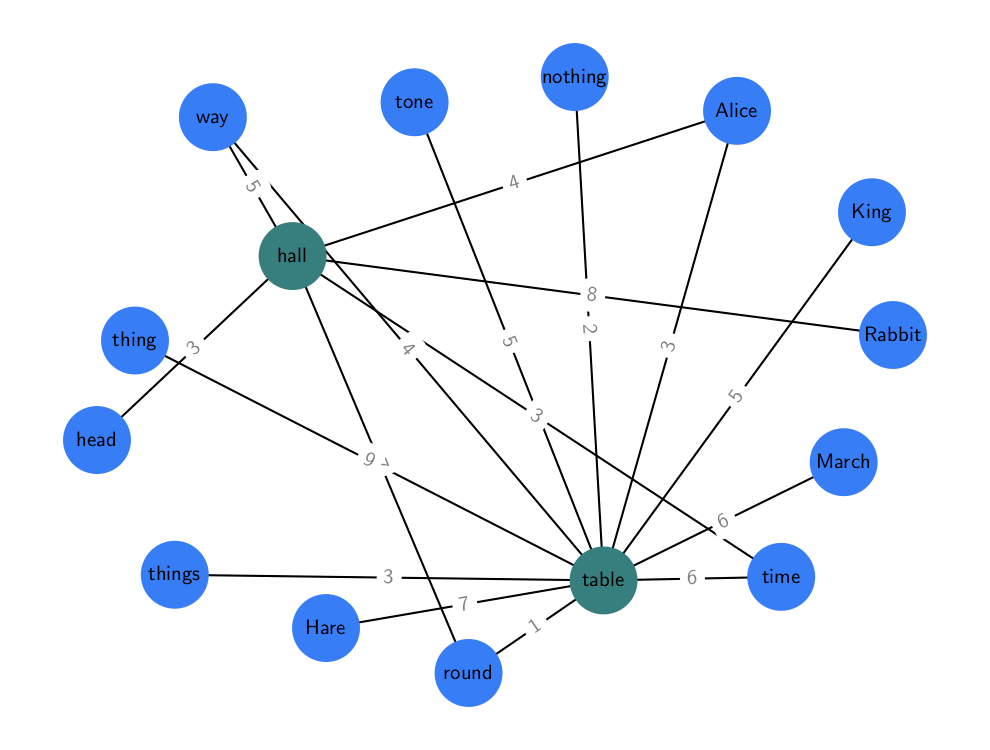
\includegraphics[width=0.6\textwidth]{Images/aiw_composite_mapped.png}
    \caption{Sample mapping of composite tokens (green) to basis tokens (blue) in AIW.}
    \label{fig:aiw_composite_map}
\end{figure}
